\documentclass[aspectratio=169, 11pt]{beamer}

% --- Packages & Setup ---
\usepackage[utf8]{inputenc}
\usepackage[T1]{fontenc}
\usepackage{helvet}
\renewcommand{\familydefault}{\sfdefault}
\usepackage{xcolor}
\usepackage{booktabs}
\usepackage{graphicx}
\usepackage{tikz}
\usetikzlibrary{calc}

\graphicspath{{../figures/}{./}}

% --- Branding Colors ---
\definecolor{amritaMaroon}{HTML}{A4123F}

% --- Theme Setup ---
\usetheme{Madrid}
\usecolortheme[named=amritaMaroon]{structure}
\setbeamertemplate{navigation symbols}{}
\setbeamertemplate{footline}[frame number]

\begin{document}
\begin{frame}
    \begin{tikzpicture}[remember picture,overlay]
        \node[fill=amritaMaroon, text=white, font=\bfseries\footnotesize, anchor=north east, rounded corners=2pt, inner sep=5pt]
        at ($(current page.north east) + (-0.2cm,-0.2cm)$) {Type 2: Application Project};
    \end{tikzpicture}
    \centering
    
\includegraphics[width=2.8cm]{logo.png}
    \vspace{0.1cm}

    {\large \textbf{\textcolor{amritaMaroon}{Court-Calibrated Group Activity Recognition for Volleyball Team Behaviour Analysis Using Monocular Video}}} \\
    \vspace{0.05cm}
    {\footnotesize \textbf{23CSE498 -- Project Phase II (External Review)} \quad | \quad \textbf{Team Number: 56}} \\
    \vspace{0.1cm}
    \begin{table}
        \centering
        \scriptsize
        \renewcommand{\arraystretch}{1.0}
        \begin{tabular}{|c|c|l|}
            \hline
            \textbf{S.No} & \textbf{Register Number} & \textbf{Student Name} \\
            \hline
            1 & CB.SC.U4CSE23415 & G. Bharath Chandra \\
            \hline
            2 & CB.SC.U4CSE23420 & K. Surya Sekhar \\
            \hline
            3 & CB.SC.U4CSE23425 & Keshavramprakash D. \\
            \hline
            4 & CB.SC.U4CSE23453 & U. Yeshwanth Kumar Reddy \\
            \hline
            5 & CB.SC.U4CSE23768 & V. Punith Sai \\
            \hline
        \end{tabular}
    \end{table}
    \vspace{0.05cm}
    {\footnotesize Guide: \textbf{Dr. Divya Singh}, Assistant Professor, Department of CSE} \\
    \vspace{0.05cm}
    {\scriptsize \today}
\end{frame}

\begin{frame}{Guide Review \& Submission Approval}
    \framesubtitle{Confirmation of Project Review and Approval from Guide}
    \centering
    \IfFileExists{guide_approval.png}{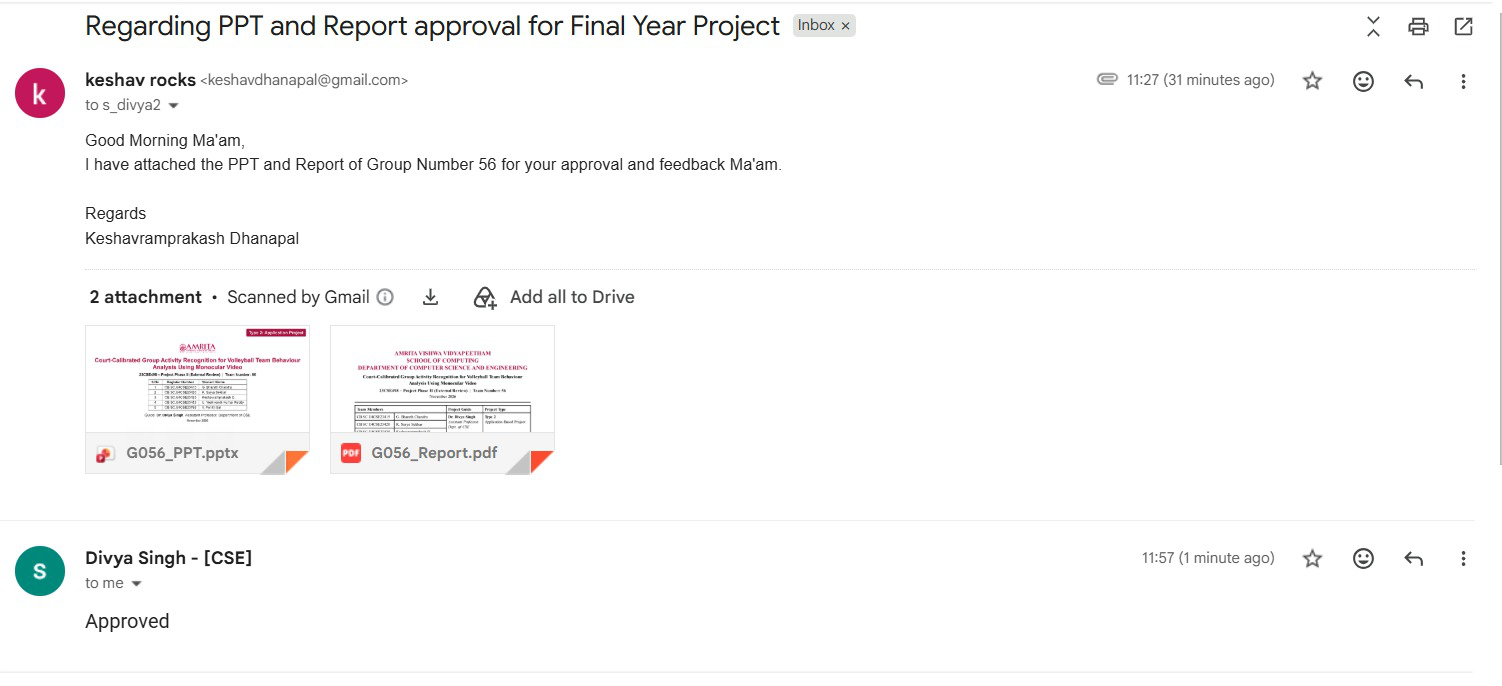
\includegraphics[height=5.6cm]{guide_approval.png}}{%
    \fbox{\begin{minipage}[c][5.4cm]{0.94\textwidth}
        \centering
        \textbf{[Insert Screenshot of Guide Approval Email Here]} \\[0.3cm]
        {\footnotesize Save the screenshot as guide\_approval.png next to this file and recompile.}
    \end{minipage}}}
\end{frame}

\begin{frame}{1. Problem Definition \& Requirement Analysis}
    \framesubtitle{Target Problem, User Needs \& Functional / Non-Functional Requirements}
\begin{block}{Problem Statement \& Target Stakeholders}
\scriptsize
\begin{itemize}
  \item \textbf{Real-World Problem:} Coaches watch match videos by hand to see how their team moves together. It takes hours, and two people can judge the same rally differently.
  \item \textbf{Target Users:} Volleyball coaches, analysts and players at clubs and colleges, who usually have only one camera and no tracking equipment.
\end{itemize}
\end{block}
\begin{block}{Functional Requirements}
\scriptsize
\begin{itemize}
  \item \textbf{FR-1:} Upload a match video (MP4, MOV, AVI, MKV, WebM) and choose the part to analyse.
  \item \textbf{FR-2:} Find and track players and the ball; give the near-side team one of 4 tactics for every second of play.
  \item \textbf{FR-3:} Show an annotated video and give downloadable reports: tactic timeline and opponent SERVE / SPIKE / BLOCK.
  \item \textbf{FR-4:} Keep a list of each user's past analyses.
\end{itemize}
\end{block}
\begin{block}{Non-Functional Requirements \& Constraints}
\scriptsize
\begin{itemize}
  \item \textbf{NFR-1:} Refuse wrong or non-volleyball files early with a clear message; show progress while working.
  \item \textbf{NFR-2:} Run on a normal laptop with a graphics card (NVIDIA RTX 3050); one camera, no sensors.
\end{itemize}
\end{block}
\end{frame}

\begin{frame}{2. End-to-End Application Architecture}
    \framesubtitle{System Architecture \& User-to-Backend Workflow Diagram}
\centering
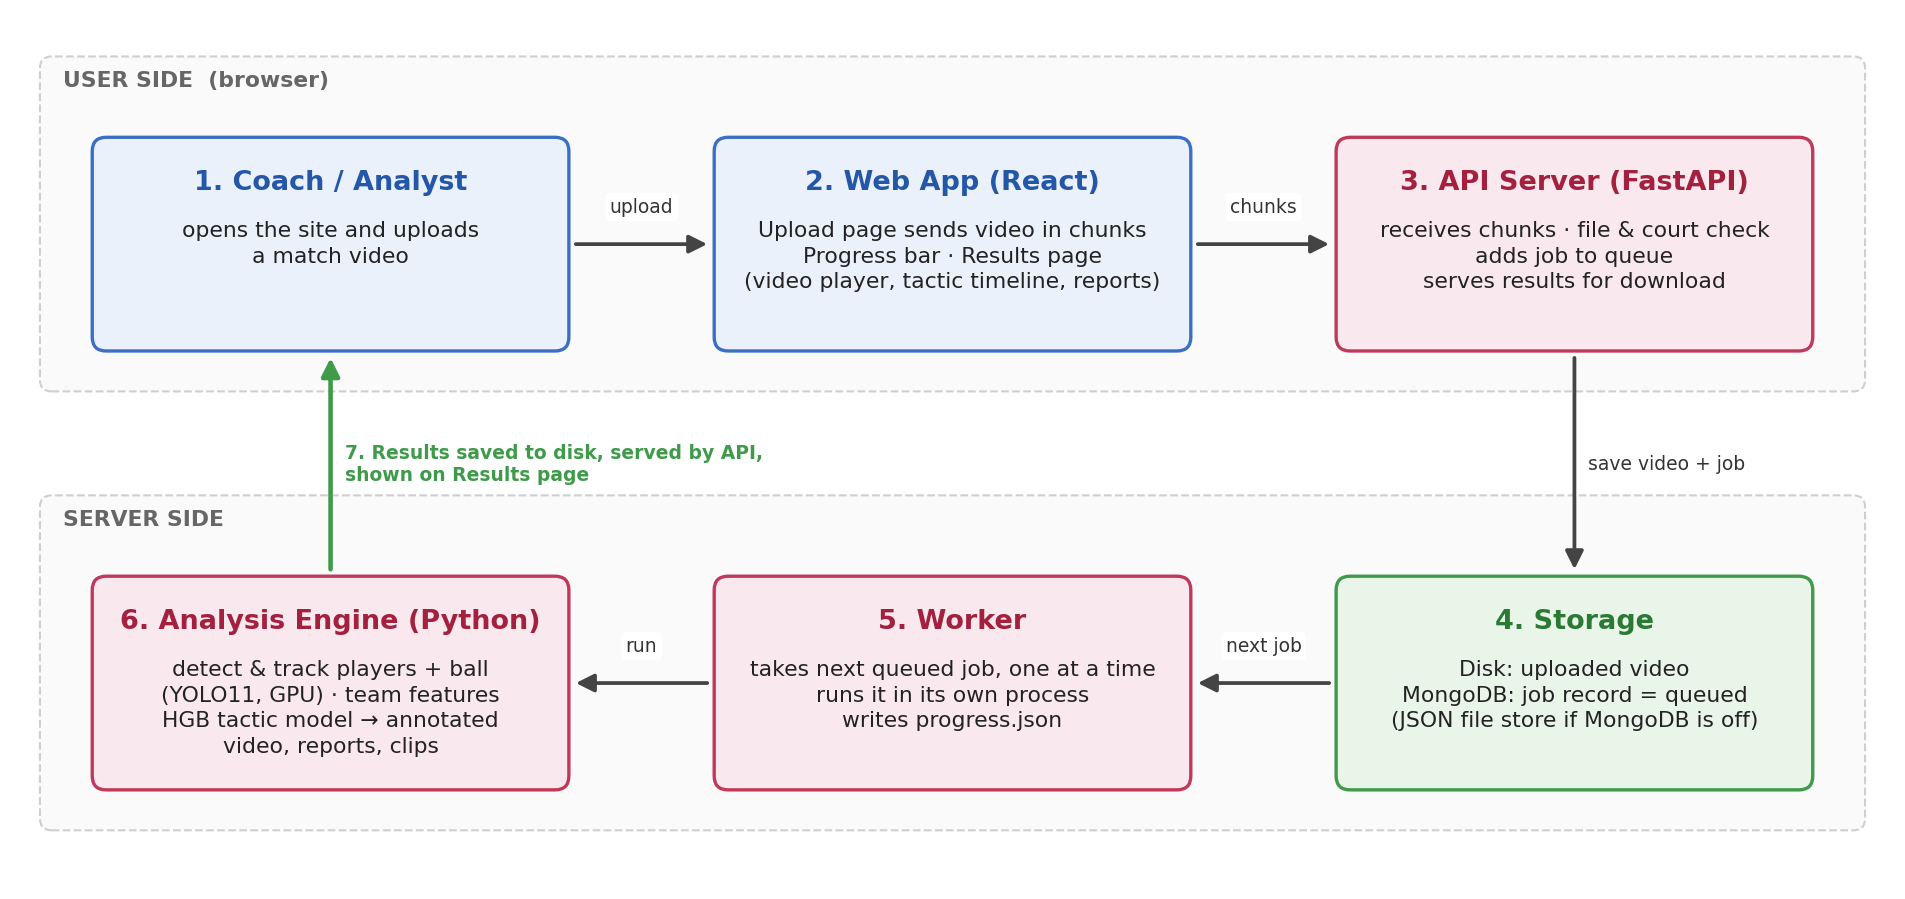
\includegraphics[width=0.97\textwidth]{web_flow_loop.png}
\vspace{0.2cm}
\begin{block}{Summary}
\footnotesize The coach uploads a video on the website. The server checks it and puts it in a queue. A worker runs the analysis one job at a time, and the results page shows the video and reports.
\end{block}
\end{frame}

\begin{frame}{2. End-to-End Application Architecture (contd.)}
    \framesubtitle{Analysis Pipeline inside the Engine}
\begin{columns}[T]
\column{0.62\textwidth}
\centering
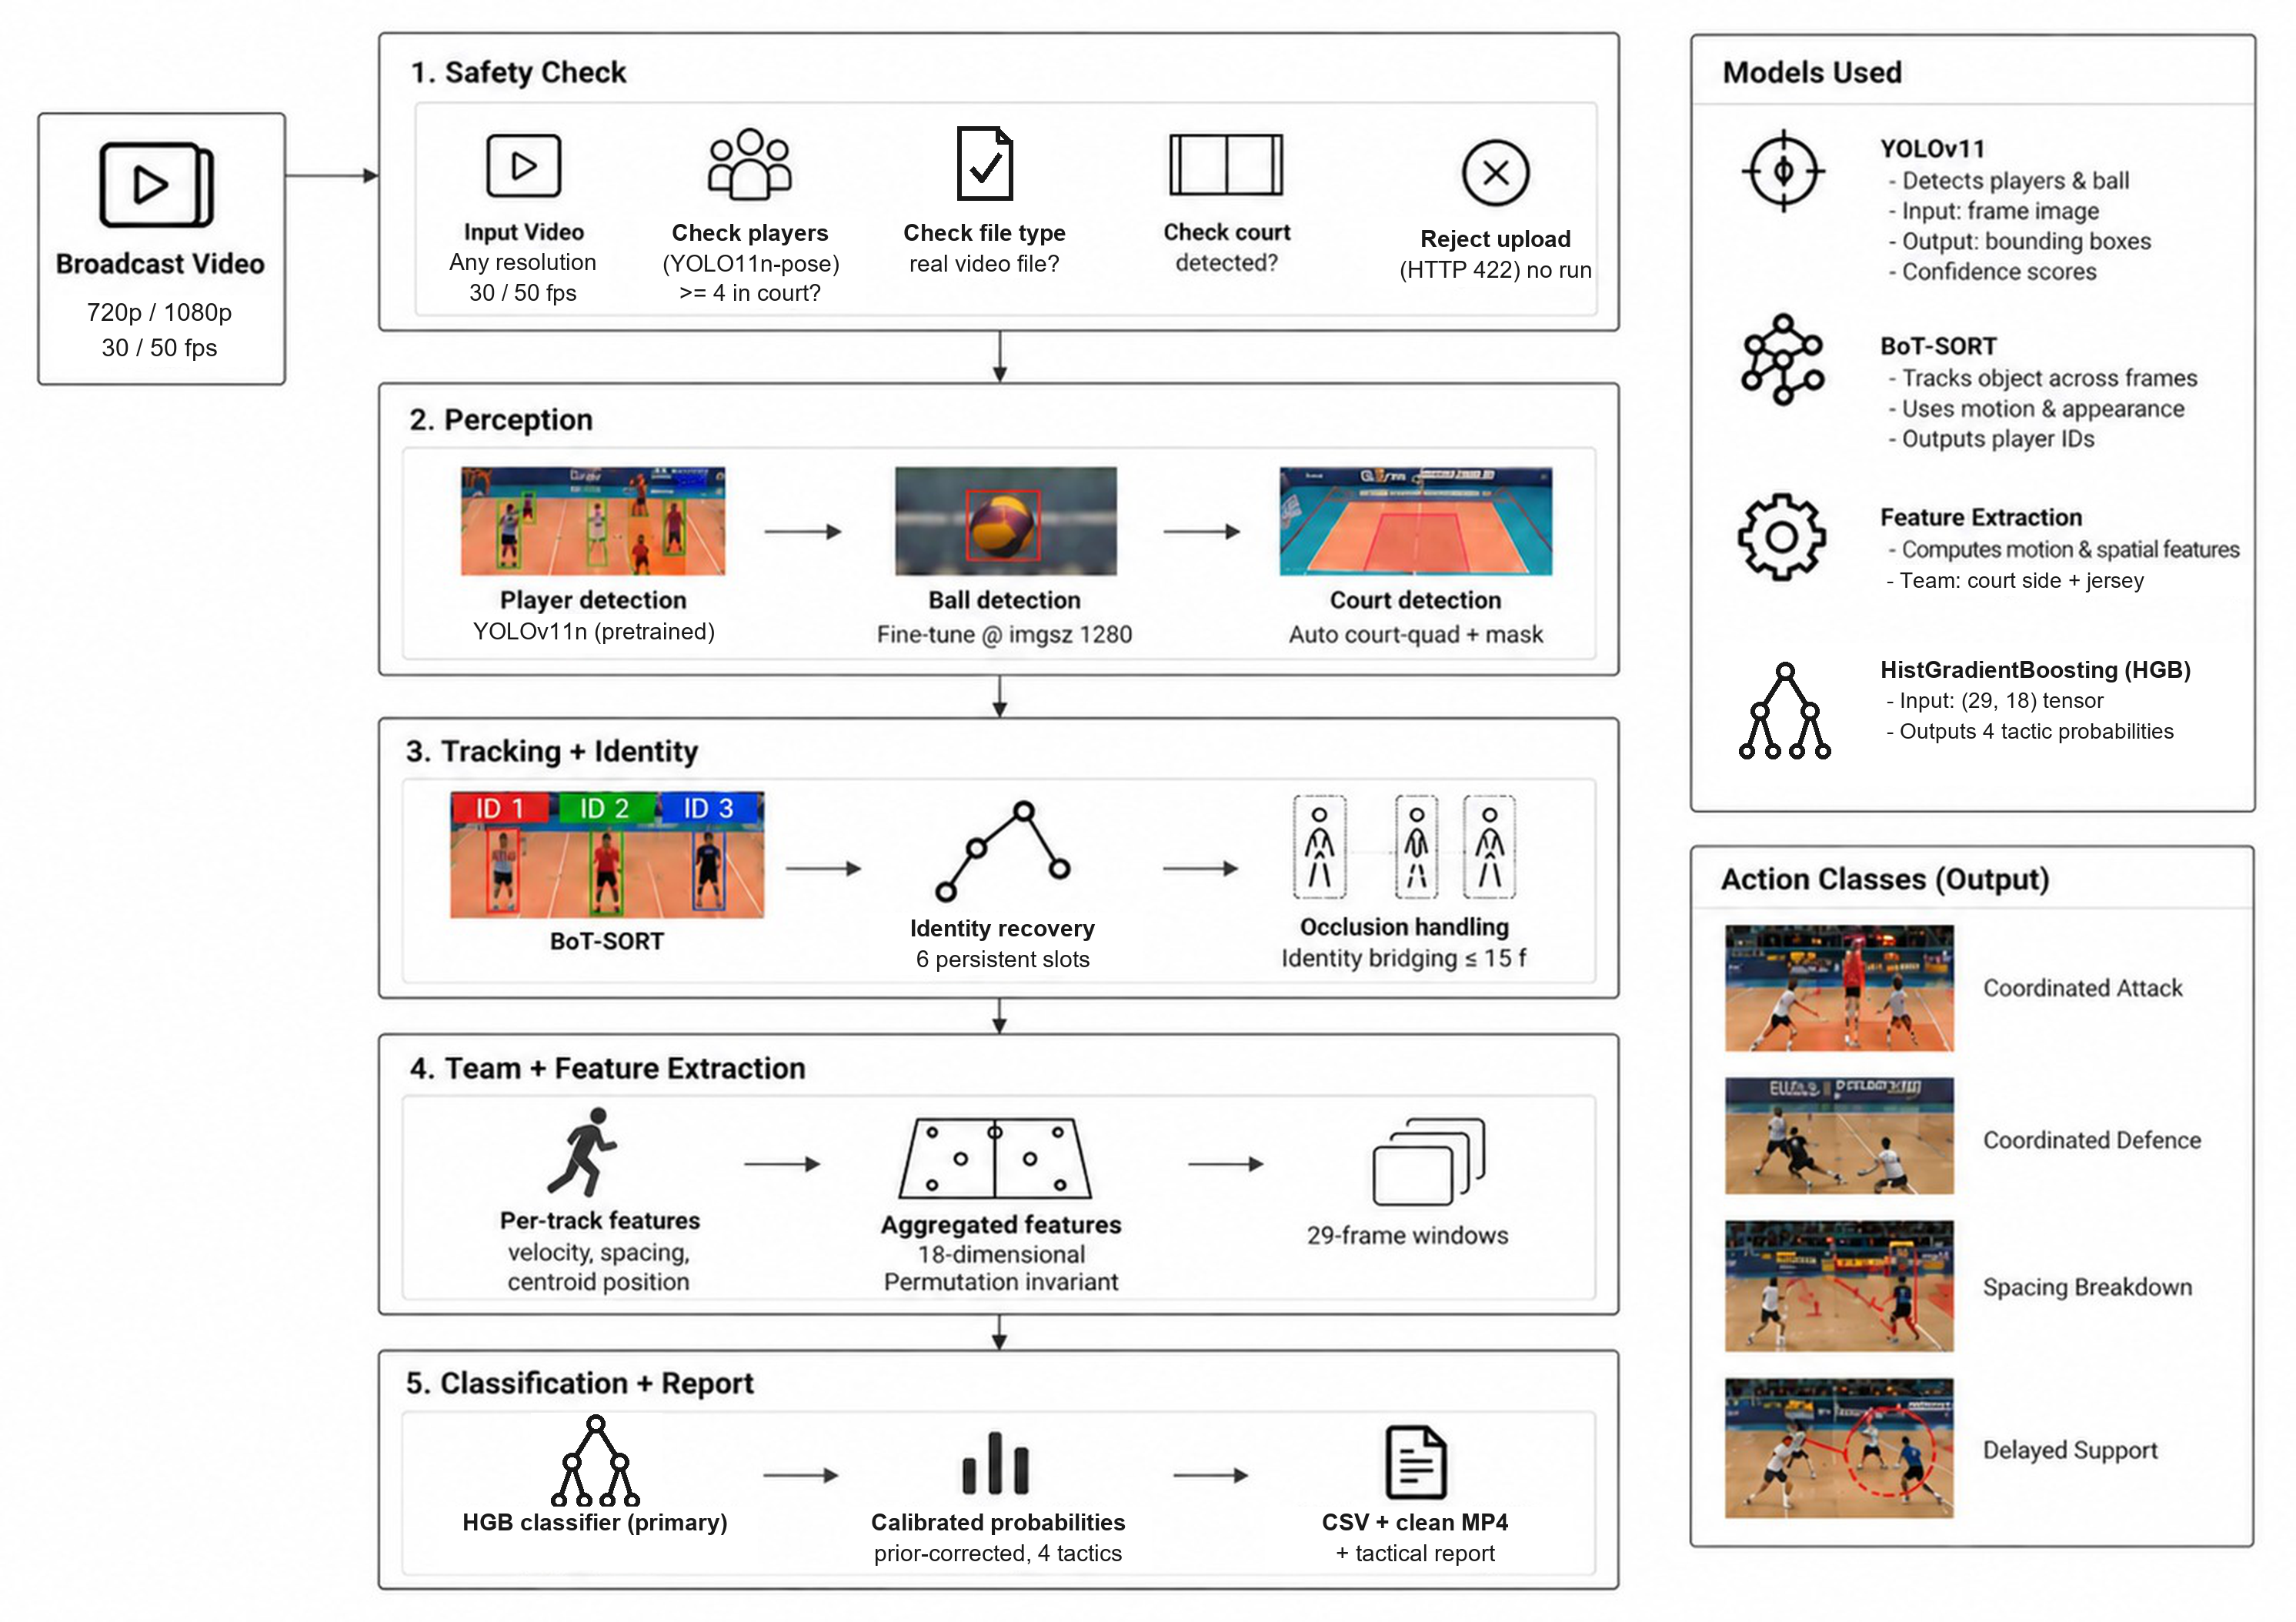
\includegraphics[width=\textwidth]{analysis_pipeline.png}
\column{0.36\textwidth}
\begin{block}{Steps in Simple Words}
\scriptsize
\begin{itemize}
  \item \textbf{1. Safety check:} is it a real video, with a court and players?
  \item \textbf{2. Detection:} find the players, the ball and the court lines.
  \item \textbf{3. Tracking:} give each player the same ID in every frame.
  \item \textbf{4. Team + features:} split the two teams; measure spacing, speed and ball position each second.
  \item \textbf{5. Tactic + report:} the HGB model names the tactic; we save the video and reports.
\end{itemize}
\end{block}
\end{columns}
\end{frame}

\begin{frame}{3. Architectural Components \& Interface Design}
    \framesubtitle{Component Breakdown, Data Flow \& Technology Specifications}
\begin{columns}[T]
\column{0.50\textwidth}
\begin{block}{Core Application Components}
\scriptsize
\begin{itemize}
  \item \textbf{Website (React):} the pages the user sees: upload, progress, results, my analyses.
  \item \textbf{Server (FastAPI):} receives the video, checks it and keeps the job queue.
  \item \textbf{Analysis Engine (Python):} finds players and ball, names the tactic, makes the output video.
\end{itemize}
\end{block}
\begin{block}{User Interaction \& Workflow Design}
\scriptsize
\begin{itemize}
  \item \textbf{User Journey:} Home, then Analyze (upload, pick time range and mode), then Progress, then Results.
  \item \textbf{Results Page:} play the annotated video, see the tactic timeline, download the reports.
\end{itemize}
\end{block}
\column{0.48\textwidth}
\begin{block}{Data Management \& External Interfaces}
\scriptsize
\begin{itemize}
  \item \textbf{Data Storage:} MongoDB keeps one record per analysis; the video and reports are saved in a folder.
  \item \textbf{External Parts:} graphics card (GPU) for fast detection; FFmpeg to make the output video.
\end{itemize}
\end{block}
\begin{block}{Platform \& Deployment Specifications}
\scriptsize
\begin{itemize}
  \item \textbf{Tools Used:} Python, FastAPI, React, MongoDB, YOLO11, scikit-learn, OpenCV, FFmpeg.
  \item \textbf{Runs On:} Windows laptop with an RTX 3050 graphics card; also as a desktop app.
\end{itemize}
\end{block}
\end{columns}
\end{frame}

\begin{frame}{4. Implementation Details -- Overview}
    \framesubtitle{End-to-End Application Module \& Integration Status}
\begin{table}
    \centering
    \scriptsize
    \renewcommand{\arraystretch}{1.2}
    \begin{tabular}{p{3.2cm} p{7.4cm} c}
        \toprule
        \textbf{Application Module} & \textbf{Implemented Features \& Integration Scope} & \textbf{Status} \\
        \midrule
Module 1: User Interface & Home, Analyze, Progress, Results, My analyses, Demos, Methodology, Documentation and Team pages; desktop app. & Complete \\
Module 2: Core Analysis & Video check, player and ball detection, tracking, team split, tactic model, opponent actions, output video, reports and clips. & Working; known accuracy limits \\
Module 3: Data \& Storage & A database record and a folder for every analysis; old analyses deleted after 14 days. & Complete \\
Module 4: External Integration & Graphics card for fast detection, FFmpeg for video, public project website; Azure CPU cloud server. & Complete (GPU cloud: future) \\
        \bottomrule
    \end{tabular}
\end{table}
\begin{block}{Prototype Environment \& Repository}
\scriptsize
\begin{itemize}
  \item \textbf{Execution Platform:} Windows 11 laptop with an RTX 3050 graphics card. One script, run\_website.bat, starts everything and opens the website.
  \item \textbf{Source Repository:} github.com/Yeshwanthreddy7/volleyball-tactical-intelligence-fyp (version 1.0.0).
\end{itemize}
\end{block}
\end{frame}

\begin{frame}{5. Functional Module Implementation Details}
    \framesubtitle{Key Feature Implementation \& Inter-Module Integration}
\begin{columns}[T]
\column{0.52\textwidth}
\begin{block}{Video Upload \& Check}
\scriptsize
\begin{itemize}
  \item \textbf{How it works:} the video is sent in small parts with a progress bar; the server then checks a few frames for a court with players.
  \item \textbf{Input \& Output:} video, time range and mode in; a job number out, or a clear error message.
  \item \textbf{Checks:} only video files; size limit; must show a volleyball court; only the uploader can cancel or delete.
\end{itemize}
\end{block}
\begin{block}{Tactic Analysis Engine}
\scriptsize
\begin{itemize}
  \item \textbf{How it works:} find players and ball, follow them, split the teams, measure the team every second, then the model names the tactic. Replays are skipped.
  \item \textbf{Connection:} runs separately from the website, so the website keeps working while a video is analysed.
\end{itemize}
\end{block}
\column{0.46\textwidth}
\centering
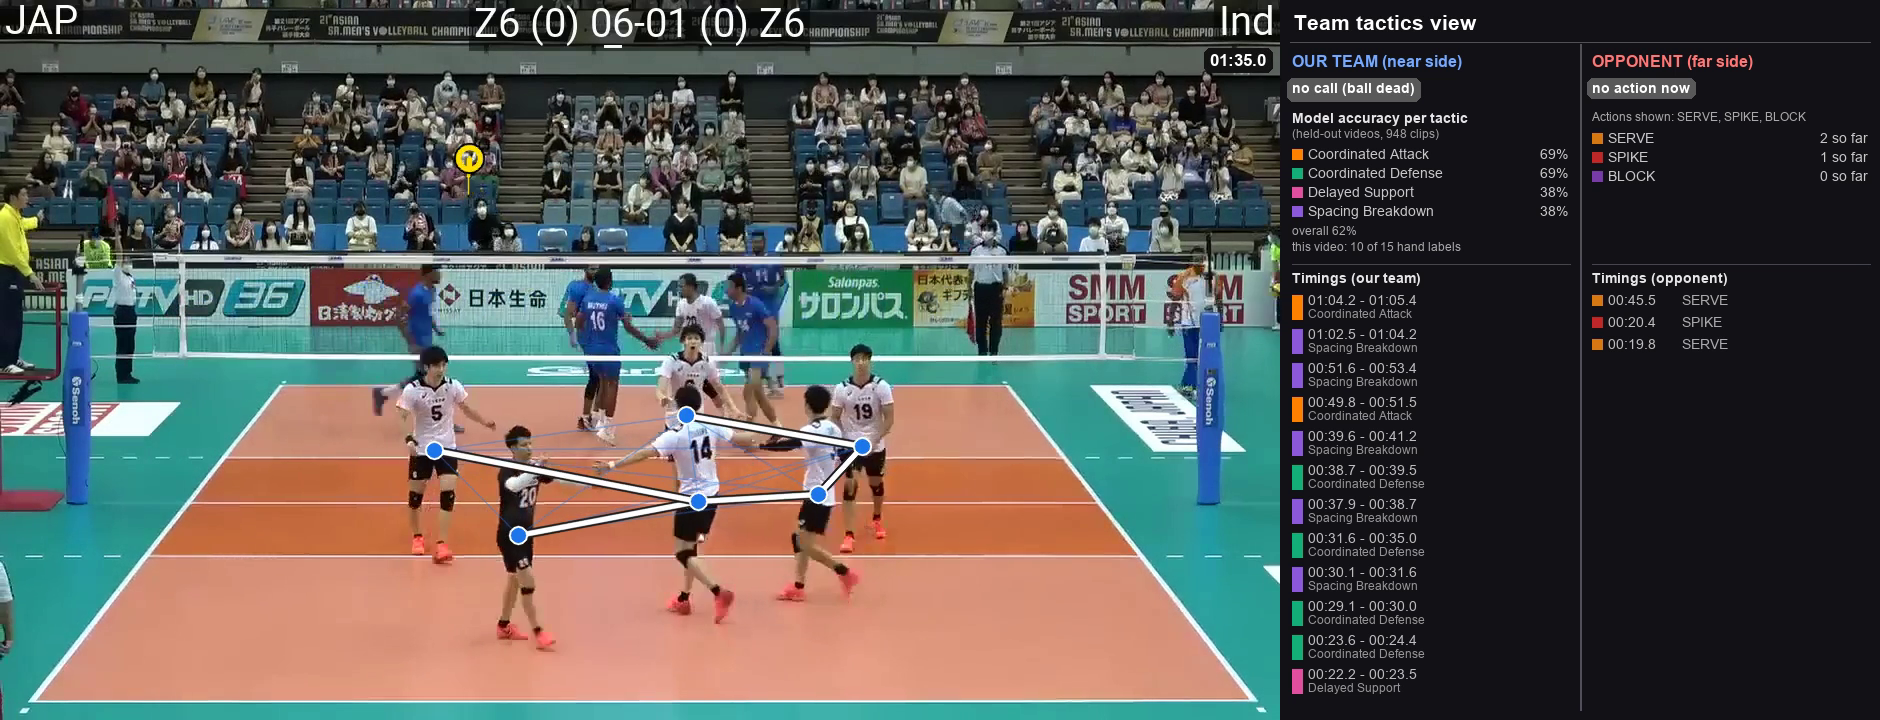
\includegraphics[width=\textwidth]{output_frame.png}\\[0.1cm]
{\scriptsize Output frame: player links, ball and tactic for the near-side team}
\end{columns}
\end{frame}

\begin{frame}{5. Functional Module Implementation Details (contd.)}
    \framesubtitle{Tactic Model and Outputs}
\begin{columns}[T]
\column{0.52\textwidth}
\begin{block}{Tactic Model}
\scriptsize
\begin{itemize}
  \item \textbf{What it does:} names the team's tactic every second: Coordinated Attack, Coordinated Defense, Delayed Support or Spacing Breakdown.
  \item \textbf{Why HGB:} we compared 16 models; HGB was among the most accurate and runs fast, even without a graphics card.
\end{itemize}
\end{block}
\begin{block}{Outputs}
\scriptsize
\begin{itemize}
  \item \textbf{User gets:} annotated video with sound, tactic report, opponent SERVE / SPIKE / BLOCK report, and short example clips.
\end{itemize}
\end{block}
\column{0.46\textwidth}
\centering
{\scriptsize \textbf{Accuracy on videos never seen in training}}\\[0.1cm]
\scriptsize
\begin{tabular}{llr}
\toprule
\textbf{Model} & \textbf{Type} & \textbf{Correct Tactic} \\
\midrule
HGB (our model) & Machine learning & 63.7\% \\
InceptionTime & Deep learning & 61.9\% \\
Mamba & Deep learning & 46.1\% \\
Guessing the most common tactic & Baseline & 39.0\% \\
\bottomrule
\end{tabular}\\[0.1cm]
{\tiny 945 clips from 8 videos; each video tested once while the model trained on the other 7.}
\end{columns}
\end{frame}

\begin{frame}{6. Functional Testing \& Verification Results}
    \framesubtitle{End-to-End Feature Verification \& Test Case Summary}
\begin{table}
    \centering
    \tiny
    \renewcommand{\arraystretch}{1.15}
    \begin{tabular}{p{3.0cm} p{3.4cm} p{4.4cm} c}
        \toprule
        \textbf{Test Case / Feature} & \textbf{Test Input / Action} & \textbf{Verified Outcome} & \textbf{Status} \\
        \midrule
TC-01: Full analysis & 150-second match video, Accurate mode & annotated video, 40 tactic segments, 9 opponent actions, clips for all 4 tactics & Pass \\
TC-02: Real match check & all 11 match videos in our dataset & all accepted & Pass \\
TC-03: Not volleyball & street photo, test pattern, screen recording & refused with a clear message & Pass \\
TC-04: Wrong file type & a PDF document & refused; allowed types shown & Pass \\
TC-05: Fake video file & a text file renamed to .mp4 & detected and refused & Pass \\
TC-06: File too large & a 5 GB file & refused before upload starts & Pass \\
TC-07: Security check & asked for a missing analysis and a hidden server file & refused; nothing shown & Pass \\
TC-08: Automated tests & 266 automatic code checks & all 266 passed & Pass \\
        \bottomrule
    \end{tabular}
\end{table}
\begin{block}{Application Verification Summary}
\scriptsize
\begin{itemize}
  \item \textbf{Testing:} all 8 test cases passed, and 3 full analyses finished on the laptop.
  \item \textbf{Speed \& Accuracy:} about 7 minutes per minute of video on the laptop. On videos the model never saw, it is right 63.7\% of the time (macro-F1 0.54), against 39.0\% by guessing. Attack and Defense are reliable (F1 about 0.76); Delayed Support and Spacing Breakdown are not yet (F1 about 0.3).
\end{itemize}
\end{block}
\end{frame}

\begin{frame}{7. Working Prototype Demonstration}
    \framesubtitle{End-to-End Application Walkthrough \& Visual Evidence}
\begin{columns}[T]
\column{0.48\textwidth}
\centering
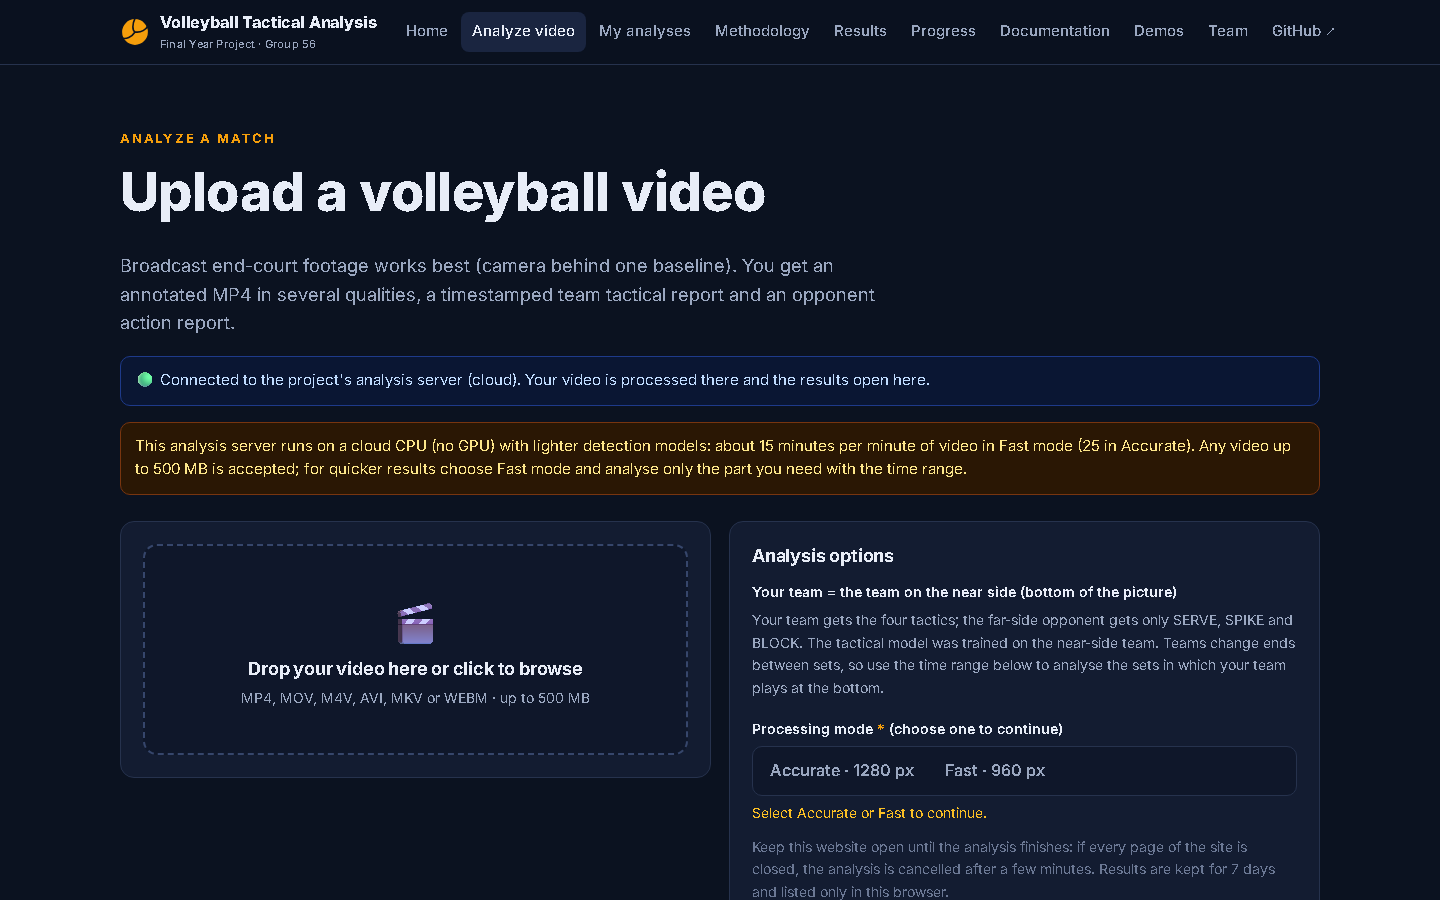
\includegraphics[width=\textwidth,height=4.3cm,keepaspectratio]{site_analyze.png}\\
{\scriptsize Input view: upload page with mode choice}
\column{0.48\textwidth}
\centering
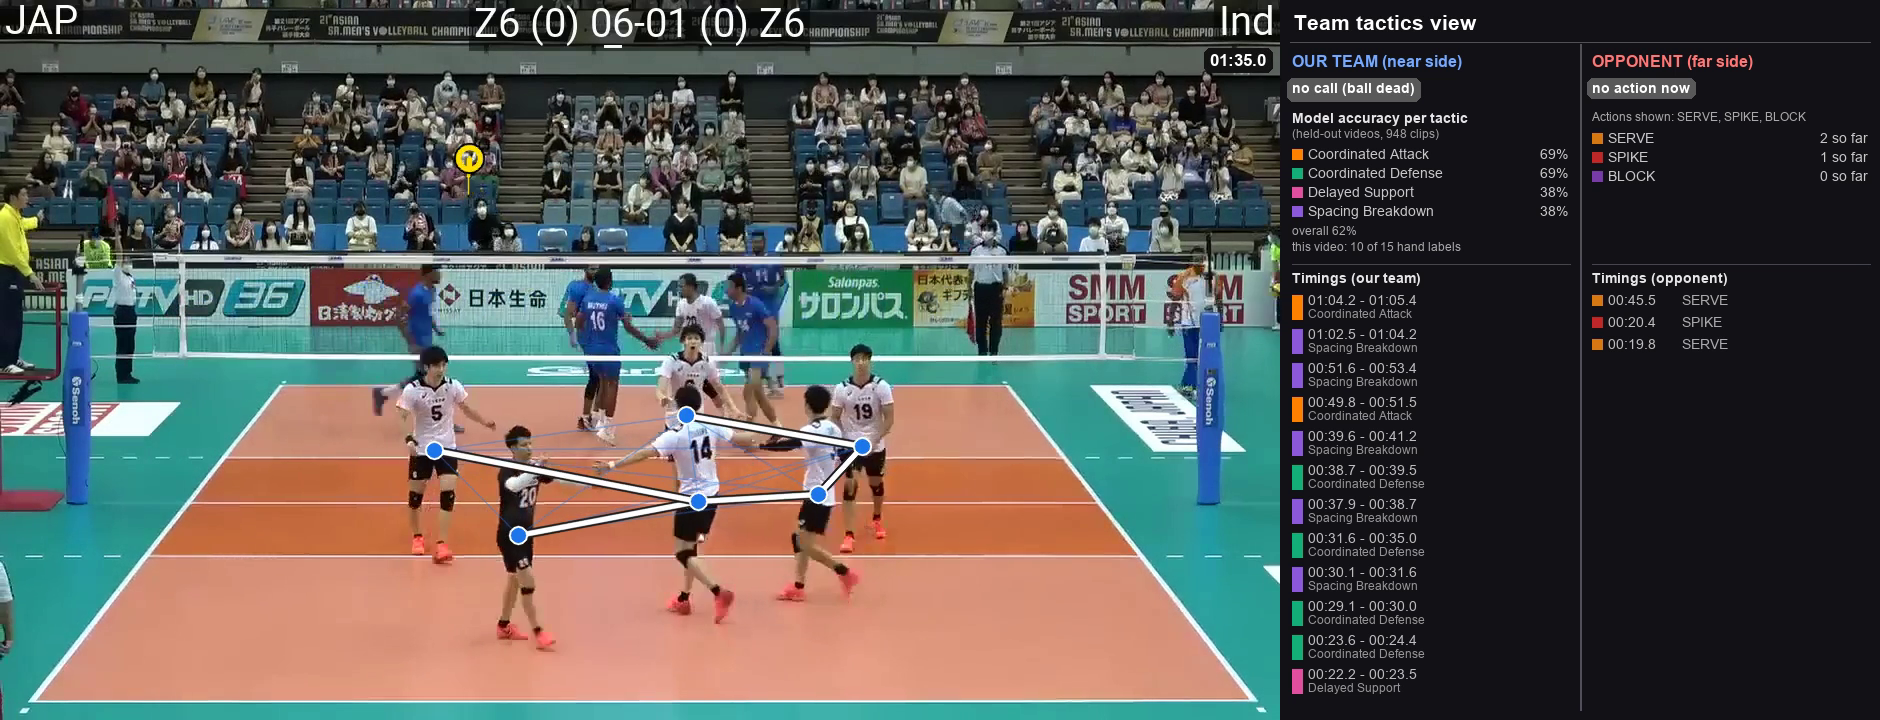
\includegraphics[width=\textwidth,height=4.3cm,keepaspectratio]{output_frame.png}\\
{\scriptsize Output view: annotated match video}
\end{columns}
\vspace{0.2cm}
\begin{block}{Live Demonstration Scenario}
\footnotesize We open the website on the laptop, upload a one-minute match clip, choose Accurate mode and watch the progress bar. Then we play the annotated video, show the tactic timeline and download the reports.
\end{block}
\end{frame}

\begin{frame}{8. Technical Justification \& Architectural Decisions}
    \framesubtitle{Platform Rationale, Engineering Trade-offs \& Operational Considerations}
\begin{columns}[T]
\column{0.48\textwidth}
\begin{block}{1. Why These Tools}
\scriptsize
\begin{itemize}
  \item Python is the standard choice for video analysis and machine learning.
  \item FastAPI handles big uploads well; React makes a fast, simple website; MongoDB stores job records easily.
\end{itemize}
\end{block}
\begin{block}{2. Design Trade-offs}
\scriptsize
\begin{itemize}
  \item One analysis at a time, so the 4 GB graphics card never runs out of memory.
  \item The analysis runs separately, so a problem in one video does not stop the website.
\end{itemize}
\end{block}
\column{0.48\textwidth}
\begin{block}{3. Security \& Error Handling}
\scriptsize
\begin{itemize}
  \item Only real video files are accepted; only the uploader can cancel or delete a job.
  \item If the page is closed, the job stops after 5 minutes; if court lines are not found, a standard court is used.
\end{itemize}
\end{block}
\begin{block}{4. Limits \& Future Scope}
\scriptsize
\begin{itemize}
  \item Works after the match, not live; covers the near-side team.
  \item Now: public site on an Azure CPU server (Fast mode). Next: a cloud server with a GPU, more match videos, better ball detection.
\end{itemize}
\end{block}
\end{columns}
\end{frame}

\begin{frame}{9. Limitations \& Future Scope}
    \framesubtitle{What the Prototype Cannot Do Yet, and What Comes Next}
\begin{columns}[T]
\column{0.48\textwidth}
\begin{block}{Current Limitations}
\footnotesize
\begin{itemize}
  \item Analysis is after the match, not live: about 7 minutes per minute of video.
  \item Tactics are given for the near-side team; teams change sides each set, so we analyse one set at a time.
  \item Delayed Support and Spacing Breakdown are recognised less reliably than attack and defense.
  \item The model learned from 945 clips of 8 match videos labelled by one annotator; more data and a second annotator will help.
  \item Opponent SERVE / SPIKE / BLOCK rules were right in 17 of 31 hand-checked events; missed events are not yet counted.
\end{itemize}
\end{block}
\column{0.48\textwidth}
\begin{block}{Future Scope}
\footnotesize
\begin{itemize}
  \item Run the website on a cloud server with a graphics card for faster results.
  \item Add more match videos and labels to improve accuracy.
  \item Finish the new ball detector, now being trained on all 11 videos.
  \item Recognise team names and follow the same team across sets.
\end{itemize}
\end{block}
\end{columns}
\end{frame}

\section{References}
\nocite{*}
\begin{frame}[allowframebreaks]{References}
    \footnotesize
    \bibliographystyle{ieeetr}
    \bibliography{ref}
\end{frame}

\begin{frame}
    \centering
    {\Huge \textbf{\textcolor{amritaMaroon}{Thank You}}} \\[0.4cm]
    {\large \textbf{Questions \& Viva Voce}}
\end{frame}

\end{document}
